\documentclass[11pt]{article}
%Gummi|065|=)
\title{\textbf{CMEE Coursework\\Week 3, Practical 9.9.2}}
\author{Calum Pennington}
\date{}

\usepackage[margin=1.5cm]{geometry}
\usepackage{graphicx}
\usepackage{caption}
\usepackage{subcaption}

\begin{document}
\maketitle

\section*{Is the temperature of one year significantly correlated with the next year (successive years), across the years?}
Spearman rank-order correlation indicates a significant positive association between the temperature of one year and the next year, across the years (\emph{$r_s$}=0.33, \emph{P}$<$0.05). A scatterplot summarises the result (Figure 1a). Overall, there is a moderate, positive correlation among temperatures in successive years. An increase on the previous year's temperature correlated with an increase the next year. The data seem to show a linear relationship: a constant increase.

'Standard' correlation (Pearson's product-moment correlation) assumes variables are normally distributed. I chose Spearman's rank-order correlation, not the Pearson, as the temperature data did not look normally distributed (Figure 1b). Climatic variables in successive time points are not independent. So, I did not use the standard p-value. Instead, I computed the correlation coefficient for successive years, and then ten thousand different randomly permuted sequences of years. The p-value is the fraction of coefficients greater than the original one.

\begin{figure}[h]
\centering
\begin{subfigure}{.5\textwidth}
	\centering
	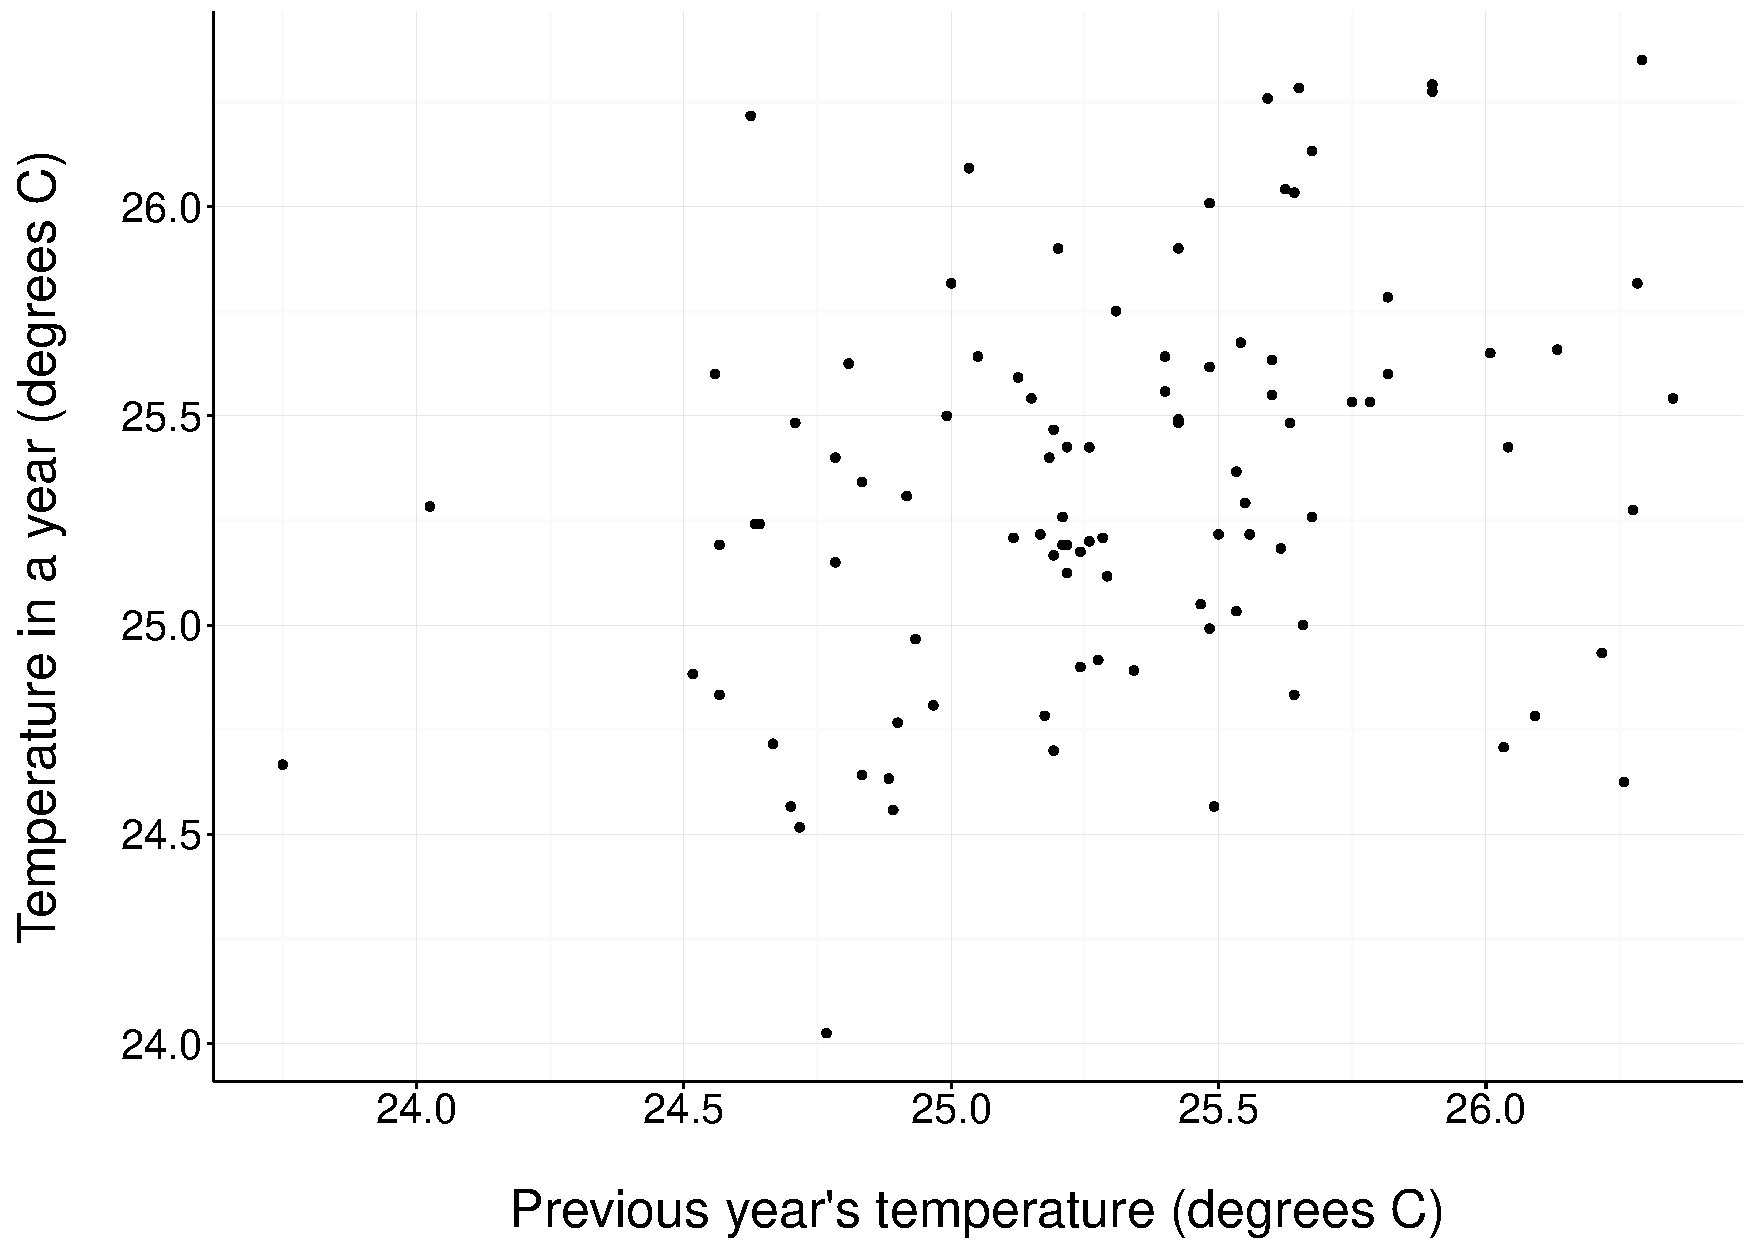
\includegraphics[width=0.8\linewidth]{../Results/AutoCorr_Scatter.pdf}
   \caption{Positive correlation between the temperature of one year and the next year, across the years.}
\end{subfigure}%
\begin{subfigure}{.5\textwidth}
  \centering
  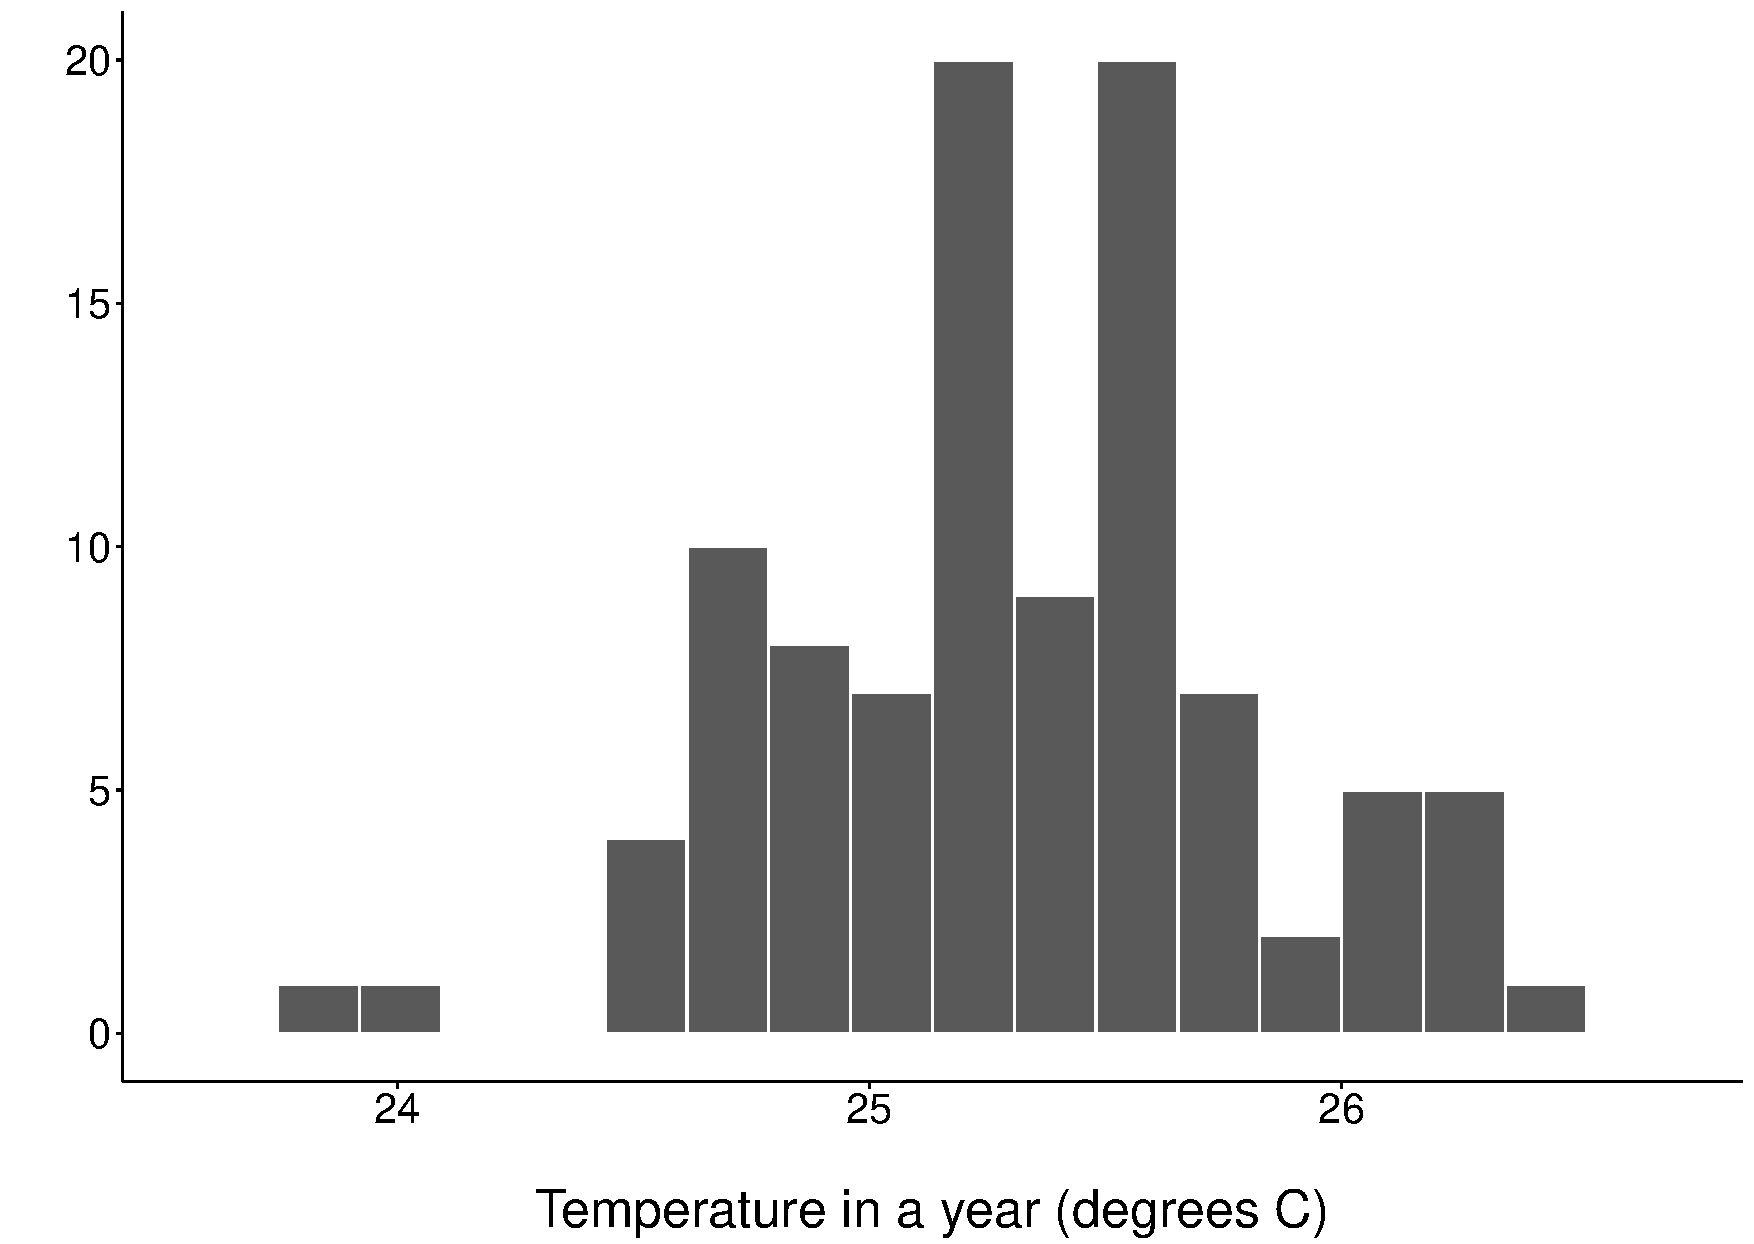
\includegraphics[width=0.8\linewidth]{../Results/AutoCorr_Hist.pdf}
  \caption{The temperature data is not normally distributed.}
\end{subfigure}
\caption{Temperature in Key West, Florida, for each year of the $20^{th}$ Century.}
\end{figure}

While there is high variability, this seems constant across the distribution and there are no outliers. This suggests there is a long term trend, independent of short term fluctuations.

Perhaps the temperature of a year is caused by the previous year. The direction of causality would be obvious: it makes no sense to think the temperature of a year affects previous years. But, at this stage, this is not a valid conclusion: correlation does not imply causality. The sample size is reasonably big: temperature for each year of the $20^{th}$ Century. The result is unlikely to be coincidental, and suggests there is a constant factor affecting the variables.

\end{document}
\grid
\grid
\grid
